\chapter{Wprowadzenie do tematyki pracy}
\label{cha:tematykaPracy}
Cyfrowa akwizycja obrazu pozwala na odwzorowanie widzialnej dla człowieka sceny w przestrzeni zdigitalizowanej. Takie przedstawienie obrazu umożliwia utrwalenie go na rozmaitych nośnikach pamięci i dostęp do niego w dowolnym momencie w przyszłości. Rejestrując zdjęcia z pewną częstotliwością i zachowaniem kolejności ich akwizycji otrzymuje się nagranie wideo. Pozwala ono śledzić zmiany na scenie następujące w czasie, takie jak ruch czy \textcolor{red}{zmiana} oświetlenia. Następujące po sobie obrazy zwane \textbf{ramkami} to \textbf{sekwencja wideo}.
\section{Preprocessing}
Choć dla człowieka informacje zawarte na obrazie są proste w interpretacji, maszyna ''widzi'' ramkę jako zwykły ciąg liczb. Dlatego aby dokonywać automatycznej detekcji pewnych zjawisk i zależności, należy poddać ją odpowiednim przekształceniom, pozwalającym wyekstrahować interesujące powiązania. Zanim jednak to się stanie, należy między innymi dokonać uwydatnienia pożądanych cech na obrazie i pozbyć się zakłóceń, czyli poddać go filtracji. Taki proces nazywa się przetwarzaniem wstępnym, czyli \textit{preprocessingiem}. Do tej fazy wliczamy m.in.:
\begin{itemize}
\item przekształcenia geometryczne, wykorzystywane do korekcji błędów urządzeń akwizycyjnych
\item przekształcenia punktowe, nie wymagające znajomości otoczenia piksela
\item przekształcenia kontekstowe - na przykład filtry, ustalające wartość piksela na podstawie poziomu jasności pikseli z nim sąsiadujących
\item przekształcenia widmowe, jak  np. transformata Fouriera
\item przekształcenia morfologiczne, modyfikujące wartość piksela przy spełnieniu pewnego warunku logicznego
\end{itemize}
W zależności od tego, jakie elementy ramki są w programie istotne, stosuje się różne metody uwydatnienia informacji. W książce \cite{i1823330731}, z której pochodzi wspomniana wyżej klasyfikacja, opisane są najczęściej wykorzystywane algorytmy używane w takim procesie. W tej sekcji zostaną przedstawione niektóre z nich, istotne w kontekście niniejszej pracy.
\subsection{Filtracja}
Filtracja obrazu ma na celu wyeliminowanie niepożądanych cech obrazu. Jest to operacja kontekstowa, a więc wymagająca informacji o jasności piksela i jego otoczenia. Staje się przez to procesem wykorzystującym duże nakłady obliczeniowe maszyny, przez co znacznie opóźnia działanie metody wykorzystującej filtrację - dlatego też istotny jest dobór jak najbardziej optymalnego sposobu eliminacji zakłóceń w zależności od danych. Dostępnych jest wiele metod, jak choćby filtracja górno- lub dolnoprzepustowa czy filtracja medianowa. Dokonuje się także klasyfikacji filtrów na liniowe (w oparciu o kombinację wartości odpowiednich pikseli obrazu wejściowego) i nieliniowe (do przekształceń wykorzystujące nieliniową funkcję odpowiednich pikseli obrazu). 
\subsubsection{Konwolucja}
Operacją wykorzystywaną przy filtrach liniowych jest splot funkcji, czyli konwolucja. Ponieważ reprezentacja obrazów w przestrzeni cyfrowej jest dyskretna, również operacja splotu, w przestrzeni liczb rzeczywistych definiowana jako całka, może być opisana za pomocą zwykłego równania sumy:
\begin{equation}
\label{eq:konwolucja}
L'(m,n) = (w x L)(m,n) = \sum_{i,j \in K} L(m-i, n-j)w(i,j)
\end{equation}
, gdzie L - obraz wejściowy, L' - efekt splotu obrazu z maską konwolucji, w - maska konwolucji, (m, n) - współrzędne piksela, dla którego wykonywana jest konwolucja jego otoczenia z maską w.\\
Przykładowy splot fragmentu obrazu z maską filtru uśredniającego 3x3:
%\begin{equation}
\label{eq:konwolucjaPrzyklad}
\[
\begin{bmatrix}
    10 & 30  & 4 \\
    20 & \textcolor{red}{0}   & 5 \\
    0  & \textcolor{red}{100} & 102 \\
    20 & 50  & 20
\end{bmatrix}
\mathrm{x}
\begin{bmatrix}
    1 & 1 & 1 \\
    1 & 1 & 1 \\
    1 & 1 & 1
\end{bmatrix}
=
\begin{bmatrix}
    x &  x  & x \\
    x & 271 & x \\
    x & 317 & x \\
    x &  x  & x 
\end{bmatrix}
\]
%\end{equation}
\subsubsection{Normalizacja}
Ponieważ w konwolucji wykonywane są operacje mnożenia i dodawania, otrzymane wartości mogą znacznie wykraczać poza zakres, jaki należy uzyskać w danej przestrzeni - najczęściej powinna być to liczba z przedziału [0, 255]. Jak łatwo zauważyć, w przykładzie \ref{eq:konwolucjaPrzyklad} tak właśnie się stało. W celu dostosowania uzyskanych liczb do wymaganego zakresu dokonuje się normalizacji. Jeśli w masce obecne są wyłącznie elementy nieujemne, każdy wynik konwolucji dzielony jest przez sumę jej elementów. Jeśli jednak współczynniki w macierzy w są zarówno dodatnie, jak i ujemne, normalizacja musi odbywać się według następującego wzoru:
\begin{equation}
L''(m,n) = \dfrac{L'(m,n)-minL'(m,n)}{maxL'(m,n)-minL'(m,n)}
\end{equation}
\subsection{Przestrzenie barw}
Przestrzeń barw to pewna matematyczna reprezentacja światła widzialnego w przestrzeni cyfrowej. W zależności od potrzeb stosowane są różne modele. Najpopularniejszymi są spotykane w urządzeniach elektronicznych trójkanałowe RGB (ang. \textit{Red Green Blue}) oraz komplementarny do niego, stosowany w druku CMYK (ang. \textit{Cyan Magenta Yellow blacK}), wykorzystujące właściwości ludzkiego wzroku determinujące sposób, w jaki człowiek odbiera barwy. Każdemu pikselowi obrazu są tu przypisane odpowiednie wartości na każdym kanale, na przykład czerwony piksel w reprezentacji RGB na kanale czerwonym (R) ma maksymalną wartość 255 (w 8-bitowej głębi kolorów), na niebieskim i zielonym po 0. Stosowane są one do łatwej do interpretacji przez człowieka reprezentacji cyfrowej kolorów na zdjęciach. Wprowadzają one jednak duże ograniczenia ze względu na ilość niesionej informacji. Akwizycja obrazu w innej przestrzeni pozwala na przykład na zastosowanie o wiele szerszego spektrum barw. Dlatego też często przy przetwarzaniu obrazów stosuje się inne modele, rozdzielające istotne dla maszyny informacje na oddzielne kanały, co umożliwia wydajniejsze i niekiedy dokładniejsze obliczenia na zdjęciach.
\paragraph{}
\begin{figure}[!htb]
\centering
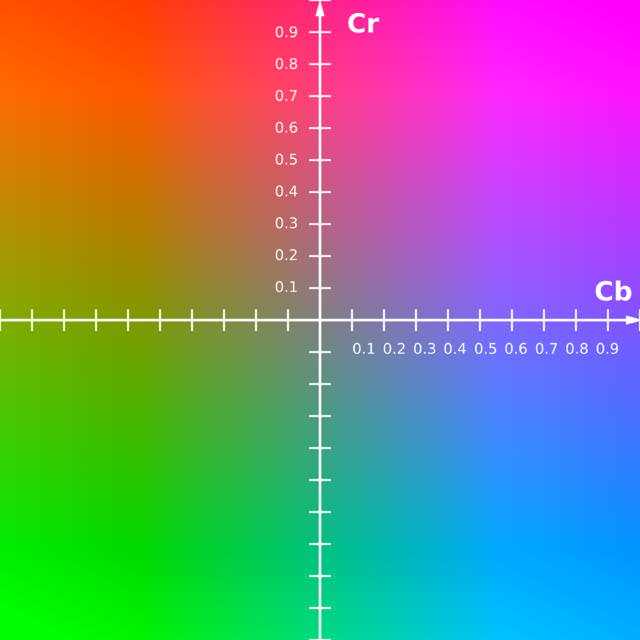
\includegraphics[width=182px]{img/YCbCr}
\caption{Reprezentacja płaszczyzny 
CbCr dla stałej luminancji Y=0.5}
%\floatfoot{Source: Wikipedia}
\end{figure}
W metodzie opisanej w rozdziale \ref{sec:BinWang}  używana jest przestrzeń YCbCr, oddzielająca kanał luminancji (Y), czyli poziomu jasności piksela, od kanałów chrominancji (Cb i Cr), przechowujących informację o jego odcieniu i nasyceniu. Taki sposób reprezentacji powstał z wykorzystaniem faktu, iż oko ludzkie jest o wiele bardziej czułe na poziom jasności obiektu, niż na jego kolor. Konwersja z przestrzeni RGB do YCbCr jest stosunkowo prosta - można ją zapisać w postaci macierzy:
%\begin{equation}

\[
\begin{bmatrix}
    Y & Cb & Cr \\
\end{bmatrix}
=
\begin{bmatrix}
    R & G & B \\
\end{bmatrix}
\begin{bmatrix}
    0.299 & -0.168935 & 0.499813 \\
    0.587 & -0.331665 & -0.418531 \\
    0.114 & 0.50059 & -0.081282 
\end{bmatrix}
\]

%\end{equation}

Ponieważ wartości na kanałach RGB mieszczą się w przedziale 0-255, po przekształceniu do przestrzeni YCbCr otrzymujemy odpowiednio wartości z przedziału [0, 255] na kanale Y oraz [-128, 127] na kanałach Cb i Cr.
\section{Analiza obrazu}  
\subsection{Binaryzacja}
Jest to jedna z podstawowych metod punktowego przetwarzania obrazu.  Pozwala odseparować istotne informacje na zdjęciu z pominięciem zależności mniej interesujących, takich jak na przykład konkretny poziom jasności, utrudniających tylko dalsze przetwarzanie ze względu na większą złożoność obliczeń. Obraz zostaje sprowadzony do postaci binarnej (zero-jedynkowej), gdzie najczęściej (w zależności od podejścia) 0 reprezentuje tło, 1 - interesujący obszar obrazu.  
\paragraph{}
Istnieje wiele metod binaryzacji, dlatego też można wybrać odpowiednią dla każdego algorytmu. Podstawowym problemem staje się jednak wyznaczenie odpowiedniego progu binaryzacji - ze względu na następującą w procesie radykalną redukcję informacji zawartych w obrazie, źle dobrany graniczny poziom jasności może doprowadzić do błędnej detekcji, w konsekwencji skutkującej złym działaniem programu. Dlatego też bardzo ważna jest znajomość rodzaju danych, z jakimi system przetwarzający będzie miał do czynienia - pozwoli to zastosować odpowiednią dla nich metodę obliczenia progu.
\subsection{Segmentacja obiektów}
Po dokonaniu binaryzacji otrzymujemy obraz czarno-biały, jednak wciąż konieczne jest przygotowanie uzyskanych wyników do dalszej analizy. Służy do tego metoda zwana segmentacją obrazu, polegająca na podziale obrazu na segmenty odpowiadające konkretnym utrwalonym na nim elementom.
\section{Detekcja ruchu na scenie}
Detekcja ruchu, czyli \textit{Motion Detection}, to sposób wykrywania przemieszczania się obiektów na scenie względem ich sąsiedztwa. Polega ona na analizie kolejnych ramek z sekwencji wideo i badaniu zmian następujących pomiędzy nimi.
\paragraph{}
Ze względu na trudność problemu detekcji, opracowanych zostało wiele metod odseparowania obiektów poruszających się od statycznych elementów sceny. Jedną z nich, stosunkowo najprostszą, jest odjęcie od obrazu wejściowego modelu uzyskanego przy pomocy algorytmów generacji tła. Na tym etapie twórcy metod muszą rozważyć jednak trzy podstawowe kwestie:
\begin{itemize}
\item czym jest model i jak się zachowuje?
\item jak dokonać inicjalizacji modelu tła?
\item w jaki sposób aktualizować model w czasie?
\end{itemize}
Związane jest to z faktem, iż bardzo rzadko na sekwencjach wideo rejestrowane są sytuacje idealne - często scenie towarzyszą zmiana oświetlenia (zwłaszcza w długotrwałym monitoringu na zewnątrz) lub szumy/zakłócenia, czego rezultatem jest, iż pomimo braku ruchu obiektów poszczególne piksele zmieniają swoją wartość - co przy standardowym podejściu polegającym na porównaniu wartości pikseli odpowiadających sobie pomiędzy ramkami skutkuje fałszywą detekcją. Rzadko również do dyspozycji są sekwencje z "czystym" obrazem tła - na próbkowanych ramkach znajdują obiekty już w ruchu, albo statyczne, jednak mogące w każdej chwili zmienić swoje położenie - jak choćby zaparkowane samochody. Zasłaniają one tło, przez do wygenerowanie prawidłowego modelu staje się bardzo trudne, a niekiedy niemożliwe. Opisane w dalszej części rozwiązania stworzone zostały z uwzględnieniem niniejszych ograniczeń.
\section{Standardowe metody generacji tła}
\subsection{Średnia bieżąca}
Algorytm średniej bieżącej to bezparametrowa metoda detekcji ruchu oparta na zależnościach statystycznych. Polega ona na analizie rozkładu prawdopodobieństwa wystąpienia pewnych wartości jasności (koloru) piksela na podstawie jego sąsiedztwa.\\
\nocite{kheng2011mean}
Średnia bieżąca (ang. \textit{mean shift}) wyznaczana jest metodą iteracyjną dla każdej próbki obrazu oddzielnie. Dla danego piksela x oblicza się średnią tymczasową m(x) z jego otoczenia, która przedstawia się wzorem:
\begin{equation}
m(x) = 
\frac{\sum_{i=1}^{n}K(x-x_{i})x_{i}}{\sum_{i=1}^{n}K(x-x_{i})}
\end{equation}
, gdzie K - kernel, w którym zawarte są wagi, z jakimi brane są pod uwagę piksele sąsiedztwa x\textsubscript{i}, n - ilość pikseli sąsiedztwa \\
Średnią bieżącą nazywamy różnicę m(x) - x.
Następnie należy sprawdzić, czy wartość piksela równa jest średniej tymczasowej, czyli czy m(x) == x. Jeśli nie - należy przypisać x = m(x) i rozpocząć wyznaczanie średniej dla nowej wartości x. Jeśli jednak tak, algorytm kończy się.\\
Jeśli średnie tymczasowe obliczane są dla wielu punktów, aktualizacja ich wartości odbywa się równocześnie w każdej iteracji.
\paragraph{}
W ten sposób otrzymana średnia bieżąca może zostać użyta do wykrywania ruchu na scenie. Tworzona jest mapa gęstości prawdopodobieństwa na podstawie histogramu kolorów obiektu w poprzedniej ramce (dla każdego piksela osobno), a następnie wyszukuje się w niej szczytowej wartości w pobliżu wcześniejszego położenia obiektu. Pozwala to na wykrycie kierunku ruchu obiektu zmieniającego położenie.
\paragraph{}
Najczęściej wspominaną wadą takiego podejścia jest konieczność używania stałej wielkości ramki, w której ma znajdować się śledzony obiekt. Niewygodne staje się więc śledzenie obiektów zmieniających rozmiar w czasie, jak np. nadjeżdżających samochodów obserwowanych z odpowiedniej perspektywy. Bardziej elastyczną wersją tej metody jest CAMSHIFT (ang. \textit{Continuous Adaptive Mean Shift}, potrafiąca dostosować się do zmian w kolorystyce obiektu, a także jego rozmiarze. Implementacja obu algorytmów dostępna jest w bibliotece OpenCV.\\ \\ \\
\begin{LARGE}
\textcolor{red}{WYNIKI DLA DYNAMIC BG}
\end{LARGE}

\subsection{Gaussian Mixture Model}
\label{sec:GMM}
Metoda ta \cite{zivkovic2004improved} opiera się na obserwacji, iż obiekty tła, przy braku przemieszczających się obiektów na scenie, wykazują pewne zależności, które mogą zostać przedstawione za pomocą modeli statystycznych. Dlatego też wyodrębnienie pikseli nie pasujących do takiego modelu wiąże się z wykryciem ruchu na scenie. Jest to stosunkowo mało skomplikowany algorytm oparty na mechanizmie subtrakcji tła.
\paragraph{}
Pierwszym etapem działania algorytmu jest wyznaczenie modelu tła. Odbywa się to na podstawie gaussowskiego rozkładu prawdopodobieństwa dla każdego piksela sceny. Estymowane wartości modelu tła otrzymywane są w wyniku analizy określonej liczby próbek w czasie t. Następnie odbywa się klasyfikacja pikseli. Jeżeli prawdopodobieństwo wystąpienia danego piksela w ramce t+n jest większe od pewnego ustalonego progu, zostaje on sklasyfikowany jako tło. W przeciwnym wypadku przypisuje się go do modelu pierwszoplanowego.\\
Głównym problemem, z jakim spotyka się ta metoda, jest problem z adaptacją do zmian na scenie, na przykład w oświetleniu.\\
Prawdopodobieństwo wystąpienia danej wartości piksela x w ramce t przy K jako liczbie gausjanów używanych w modelu dane jest następującym wzorem:
\begin{equation}
P(x_{t}) = \sum_{i=1}^{K} waga_{i,t}*g(x_{t},\mu_{i,t},\sigma_{i,t})
\end{equation}
, gdzie g(a,b,c) - funkcja gęstości prawdopodobieństwa dla rozkładu Gaussa, $\mu$ - wartość średnia, $\sigma$ - odchylenie standardowe.\\
Głównym zagadnieniem dla tej metody jest kwestia doboru próbek, na podstawie których wyznaczane jest prawdopodobieństwo. Zbyt mała bądź źle dobrana ich ilość powoduje fałszywą detekcję w przypadku znacznej zmienności tła, zbyt duża - zawyżoną tolerancję, przez co piksele pierwszoplanowe zostają niekiedy sklasyfikowane jako tło.

\subsection{ViBE}
Autorzy pracy \cite{barnich2011vibe} zaproponowali jeszcze inny sposób na dokonywanie detekcji w zmieniających się warunkach otoczenia. Zamiast modelować i przewidywać wartość piksela, postanowili oni przechowywać informację o jego wcześniejszych reprezentacjach.
\paragraph{}
ViBE (ang. \textit{VIsual Background Extractor}) porzuca koncepcję estymacji pożądanej wartości piksela na podstawie wielu globalnych próbek, mogących zawierać wartości skrajnie odbiegające od średnich wartości. Zamiast tego skupia się na badaniu podobieństwa aktualnego piksela do wartości zarejestrowanych uprzednio - przechowywanie informacji o jego historii pozwala lepiej radzić sobie w warunkach drobnego ruchu na scenie.
\subsubsection{Opis metody}
Niech piksel $x$, którego wartość w przestrzeni barwnej oznaczona jest jako $v(x)$, reprezentowany jest w czasie jako zbiór poprzednich wartości $v_{i}$:
\begin{equation}
M(x) = \left\{v_{1}, v_{2}, ..., v_{n}\right\}
\end{equation}
Klasyfikacja $x$ odbywa się poprzez zbadanie odległości $v(x)$ od każdego elementu ze zbioru $M(x)$. Jeśli jest ona mniejsza od pewnego ustalonego progu ($v(x)$ i $v_{k}$ są odpowiednio bliskie), następuje zwiększenie licznika odpowiadającego pewnemu stopniowi podobieństwa badanego piksela do swojej historii. Po przekroczeniu pewnego progu podobieństwa piksel klasyfikowany jest jako tło, dalsze sprawdzanie odległości można pominąć.
\subsection{PBAS}
\cite{hofmann2012background}
\section{Standardowe metody a dynamiczne tło}
\section{Narzędzia}
\subsection{Język C++}
\subsection{Biblioteka OpenCV}

OpenCV (ang. \textit{Open Source Computer Vision}) to dostępna od 2000 roku biblioteka, zawierająca implementacje najczęściej wykorzystywanych algorytmów wizyjnych. Jej główne zalety to dostępność na zasadach \textit{open source}, a także wieloplatformowość. Została ona napisana w języku C, jednak istnieją specjalne nakładki, pozwalające korzystać z niej także m. in. w C++, C\#, Python i języku Java. Udostępniony publicznie jest nie tylko kod źródłowy, ale także i narzędzia, pozwalające na samodzielną kompilację biblioteki, co pozwala na używanie jej w wielu środowiskach programistycznych.
\paragraph{}
Biblioteka ta zawiera ponad 2500 algorytmów zoptymalizowanych pod względem pamięciowym i obliczeniowym. Jest ciągle rozwijana, co pozwala domniemywać, iż zawarte w niej rozwiązania pozwalają maksymalnie wykorzystać możliwości sprzętowe obecnych urządzeń. Korzystanie z niej zdaje się więc być najbardziej odpowiednie dla problemu opisywanego w niniejszej pracy, jako że szybkość przetwarzania wideo jest kluczowa dla detekcji w czasie rzeczywistym.
\begin{figure}[!htb]
\centering


\includegraphics[width=82px]{img/ocv_logo}
\caption{Logo biblioteki OpenCV \cite{OpenCVLogo}}
%\floatfoot{Source: }
\end{figure}

Do rozwiązania problemu rozważanego w tej pracy użyta została biblioteka \textbf{OpenCV 2.4.9}, dostępna od 25.04.2014r.